\documentclass[]{beamer}
% Class options include: notes, notesonly, handout, trans,
%                        hidesubsections, shadesubsections,
%                        inrow, blue, red, grey, brown

% Theme for beamer presentation.
\usepackage{beamerthemesplit} 
%\usepackage{moreverb}
\usepackage{listings}

% Other themes include: beamerthemebars, beamerthemelined, 
%                       beamerthemetree, beamerthemetreebars  

\title{Data Warehousing and Data Mining Project Report}    % Enter your title between curly braces
\author{Laura Bledaite \& Martynas Pumputis}                 % Enter your name between curly braces
\institute{Free University of Bozen - Bolzano}      % Enter your institute name between curly braces
\date{\today}                    % Enter the date or \today between curly braces

\begin{document}

% Creates title page of slide show using above information
\begin{frame}
  \titlepage
\end{frame}
\note{Talk for 30 minutes} % Add notes to yourself that will be displayed when
                           % typeset with the notes or notesonly class options

\section[Outline]{}

% Creates table of contents slide incorporating
% all \section and \subsection commands
\begin{frame}
  \tableofcontents
\end{frame}


\section{Milestone 1}

\begin{frame}
  \frametitle{Description}   % Insert frame title between curly braces

  \begin{itemize}
  \item Business Domain - Climbing Gear Producer's Data Warehouse
  \item Business Processes:
    \begin{itemize}
    \item Ascent
    \item Competing
    \item Route Development
    \item Sponsorship
    \end{itemize}
  \end{itemize}
\end{frame}


\begin{frame}
  \frametitle{Conceptual Design}   % Insert frame title between curly braces

  \begin{figure}[ht!]
  \centering 
  \includegraphics[width=0.9\textwidth]{/Users/laura/Dropbox/UniBZ/DWDM/dia/ascent_fact_schema.png}
  \caption{Ascent fact schema}
  \label{fig:ascent_fact_schema}
  \end{figure}

\end{frame}

\begin{frame}
  \frametitle{Logical Design}   % Insert frame title between curly braces

  \begin{figure}[ht!]
  \centering 
  \includegraphics[width=0.9\textwidth]{/Users/laura/Dropbox/UniBZ/DWDM/dia/ascent_snowflake_schema.png}
  \caption{Ascent snowflake schema}
  \label{fig:ascent_snowflake_schema}
  \end{figure}

\end{frame}

\begin{frame}
  \frametitle{Implementation}   % Insert frame title between curly braces

  \begin{itemize}
  \item DBMS - at first PostgreSQL 9.1, changed to Oracle
  \item 
  \end{itemize}

\end{frame}

\subsection{}

\begin{frame}
  \frametitle{}   % Insert frame title between curly braces

  \begin{itemize}
  \item<1-> Point 1 (Click ``Next Page'' to see Point 2) % Use Next Page to go to Point 2
  \item<2-> Point 2  % Use Next Page to go to Point 3
  \item<3-> Point 3
  \end{itemize}
\end{frame}
\note{Speak clearly}  % Add notes to yourself that will be displayed when
                      % typeset with the notes or notesonly class options


\section{Milestone 2}

\begin{frame}[fragile]
\frametitle{Most popular query}

\lstset{
    framexleftmargin=2mm, 
    frame=shadowbox, 
    rulesepcolor=\color{blue},
    language = SQL,
    tabsize = 1}

\begin{lstlisting}
SELECT * 
FROM (
	SELECT "Year", "Crag", 
		count("RankingPoints") "Count", 
		rank() OVER (PARTITION BY "Year"
		ORDER BY count("RankingPoints") DESC) AS "Rank" 
	FROM "Ascent", "Route", "Date" 
	WHERE "Ascent"."RouteID" = "Route"."RouteID"
		AND "Ascent"."DateID" = "Date"."DateID" 
	GROUP BY "Year", "Crag"
	ORDER BY "Year", "Count" DESC) 
WHERE "Rank" < 6;
\end{lstlisting}
\end{frame}


\begin{frame}[fragile]
\frametitle{Materialized view}
\lstset{
    framexleftmargin=2mm, 
    frame=shadowbox, 
    rulesepcolor=\color{blue},
    language = SQL,
    tabsize = 1}

\begin{lstlisting}
CREATE MATERIALIZED VIEW "rcd" AS
	SELECT "Route"."RouteID","Climber"."ClimberID", 
		"Date"."DateID", "Route"."GradeID", 
		"Country", "Crag", "RankingPoints", 
		"Year", "Season"
	FROM "Ascent", "Route", "Climber", "Date" 
	WHERE "Ascent"."RouteID"="Route"."RouteID"
		AND "Ascent"."ClimberID"="Climber"."ClimberID"
		AND "Ascent"."DateID"="Date"."DateID";
\end{lstlisting}
\end{frame}

\begin{frame}
\frametitle{Performance improvement (Views)}

\begin{table}[ht!]
\begin{tabular}{|c|c|c|c|c|c|c|}
\hline
Query & Time before & Time after & Difference & Improvement\tabularnewline
\hline
\hline
1 & 00:00:00.27 & 00:00:00.24 & 00:00:00.03 & 11\% \tabularnewline
\hline 
2 & 00:00:00.05 & 00:00:00.03 & 00:00:00.02 & 40\% \tabularnewline
\hline 
3 & 00:00:00.19 & 00:00:00.09 & 00:00:00.10 & 47\% \tabularnewline
\hline 
\end{tabular}
%\caption{}
\end{table}
Time before = Time required for 1 query without using a materialized view.

Time after = Time required for 1 query when using a materizlized view.
\end{frame}

\begin{frame}[fragile]
\frametitle{Indexes}
\lstset{
    framexleftmargin=2mm, 
    frame=shadowbox, 
    rulesepcolor=\color{blue},
    language = SQL,
    tabsize = 1}

\begin{lstlisting}
CREATE INDEX route_country 
	ON "Route"("Country"); 
CREATE INDEX ascent_dateid 
	ON "Ascent"("DateID"); 
CREATE INDEX ascent_routeid 
	ON "Ascent"("RouteID");
CREATE INDEX ascent_climberid 
	ON "Ascent"("ClimberID"); 
\end{lstlisting}
\end{frame}

\begin{frame}
\frametitle{Performance improvement (Indexes)}

\begin{table}[ht!]
\begin{tabular}{|c|c|c|c|c|c|c|}
\hline
Index & $Size$(kB) & $Time_{1}$ (ms) & $Time_{2}$ (ms) & $\frac{perfImpr}{Size}$\tabularnewline
\hline
\hline
route\_country & 320 & 510 & 480 & $0.09375$\tabularnewline
\hline 
ascent\_dateid & 3072 & 510 & 460 & $0.01628$ \tabularnewline
\hline 
ascent\_routeid & 3072 & 510 & 470 & $0.01302$ \tabularnewline
\hline 
ascent\_climberid & 3072 & 510 & 470 & $0.01302$ \tabularnewline
\hline 
\end{tabular}
%\caption{}
\end{table}
$Time_{1} =$ Time required for all 3 queries without indexes.

$Time_{2} =$ Time required for all 3 queries when using indexes.
\[perfImpr = Time_{2} - Time_{1}\]
\end{frame}

\section{MSR Data Mining Challenge 2012}
\subsection{Data Cleansing}

\begin{frame}
\frametitle{Data}
\begin{itemize}
\item \textbf{Original data}

  android\_platform\_bugs.xml (51 MB )
  
  git.log.xml (2.63 GB)
\item \textbf{Modified data}

db.sqlite3
\end{itemize}
\end{frame}

\begin{frame}[fragile]
\frametitle{Original Data Example}
\lstset{
    framexleftmargin=2mm, 
    frame=shadowbox, 
    rulesepcolor=\color{blue},
    language = XML,
    tabsize = 1}
\begin{lstlisting}
<bug>
	<bugid></bugid>
	<title></title>
	<status></status>
	<owner></owner>
	<closedOn></closedOn>
	<type></type>
	<priority></priority>
	<component></component>
	<stars></stars>
	<reportedBy></reportedBy>
	<openedDate></openedDate>
	<description>..</description>
</bug>
\end{lstlisting}
\end{frame}

\begin{frame}
\frametitle{Modified Data. ER diagram}
\begin{figure}[ht!]
\centering
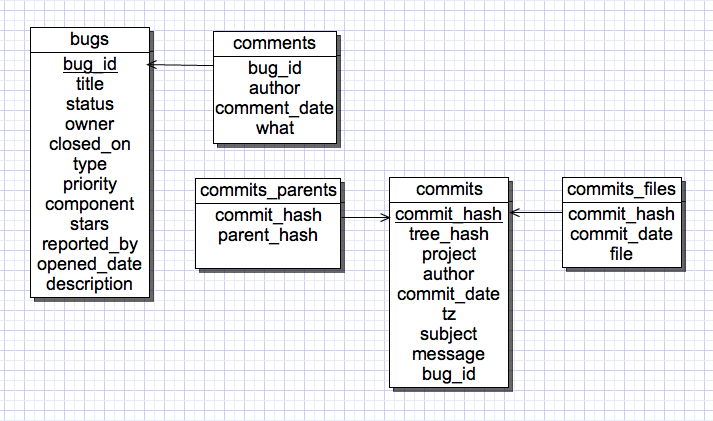
\includegraphics[width=1\textwidth]{/Users/laura/Sandbox/msr-2012/diagrams/er_diagram.png}
\end{figure}
\end{frame}

\subsection{Some Statistics}

\begin{frame}
\frametitle{Comment frequencies in a bug}
\begin{figure}[ht!]
\centering
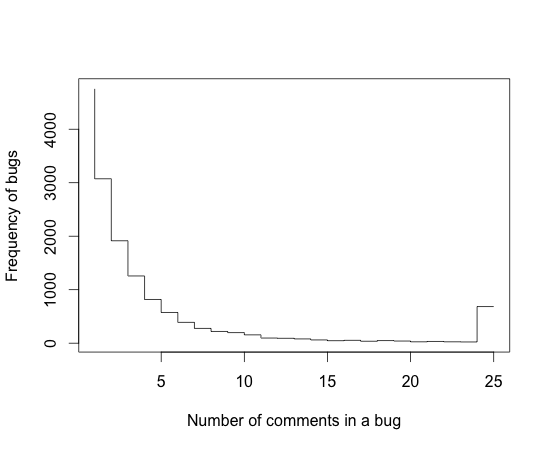
\includegraphics[width=.7\textwidth]{/Users/laura/Sandbox/msr-2012/diagrams/comment_frequencies.png}
\end{figure}
\end{frame}

\begin{frame}
\frametitle{Histogram of bug resolving times}
\begin{figure}[ht!]
\centering
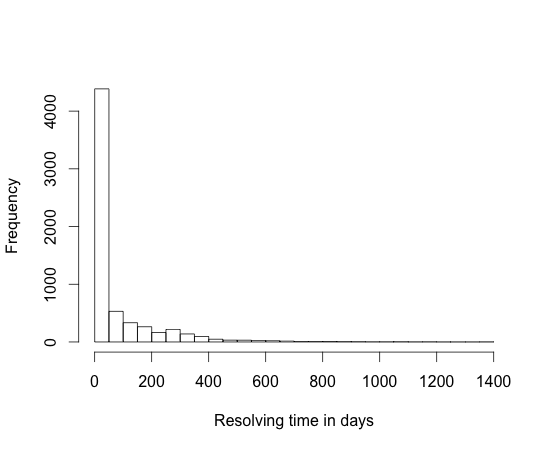
\includegraphics[width=.7\textwidth]{/Users/laura/Sandbox/msr-2012/diagrams/resolving_times.png}
\end{figure}
\end{frame}




\subsection{Buggy Files' Analysis}







\end{document}
